\documentclass[11pt,fleqn]{article} 
\usepackage[margin=0.8in, head=0.8in]{geometry} 
\usepackage{amsmath, amssymb, amsthm}
\usepackage{fancyhdr} 
\usepackage{palatino, url, multicol}
\usepackage{graphicx} 
\usepackage[all]{xy}
\usepackage{polynom} 
\usepackage{pdfsync}
\usepackage{enumerate}
\usepackage{framed}
\usepackage{setspace, adjustbox}
\usepackage{array%,tikz, pgfplots
}

\usepackage{tikz, pgfplots}
\usetikzlibrary{calc}
%\pgfplotsset{my style/.append style={axis x line=middle, axis y line=
%middle, xlabel={$x$}, ylabel={$y$}, axis equal }}
%2020 file
\pagestyle{fancy} 
\lfoot{UAF Calculus I}
\rfoot{3-3 Derivatives of Trig Functions}


\newcommand{\be}{\begin{enumerate}}
\newcommand{\ee}{\end{enumerate}}

\newcommand{\bi}{\begin{itemize}}
\newcommand{\ei}{\end{itemize}}

\begin{document}
\setlength{\parindent}{0cm}
\renewcommand{\headrulewidth}{0pt}
\newcommand{\blank}[1]{\rule{#1}{0.75pt}}
\renewcommand{\d}{\displaystyle}
\vspace*{-0.7in}
\begin{center}
 {\large{ \sc{Section 3.3 Derivatives of Trig Functions}}}
\end{center}
\begin{enumerate}
\item Use the graphs of $y = \sin x$  and $y=\cos x$ to sketch a graph of
$y'$.

\begin{tabular}{lr} 
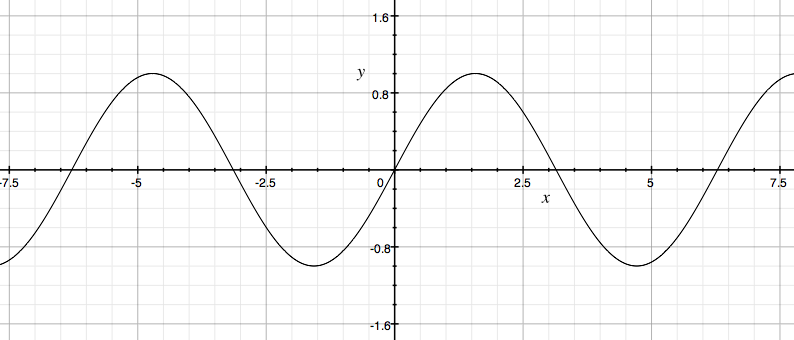
\includegraphics[width=3in]{sinx}
&
  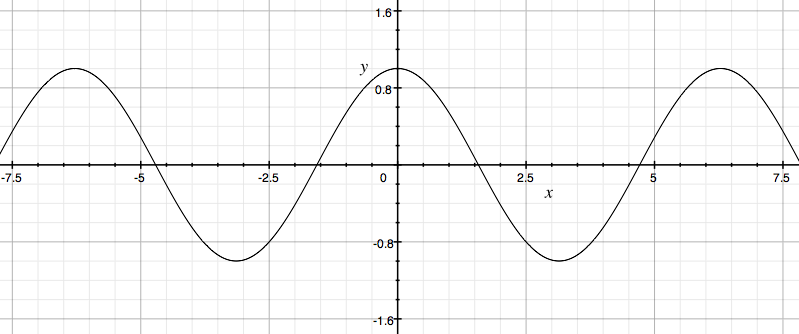
\includegraphics[width=3in]{cosx}
\end{tabular}
\item Use what we learned in 4. and 5. above to find the derivative of:
	\begin{enumerate}
	\item $y=3x^4 \cos(x)$
	\vspace{.5in}
	\item $y=\tan(x)$ (Use the Quotient Rule.)
	\vfill
	\end{enumerate}
	
	\item Fill in the table below. \\

\begin{framed}
  \textbf{Derivatives of Trigonometric Functions:}

\begin{multicols}{2}{
\vspace{-0.3in}
  \begin{itemize}
  \item $\frac{d}{dx} (\sin x) =$ \blank{0.85in}
  \item $\frac{d}{dx} (\cos x) = $ \blank{0.85in}
  \item $\frac{d}{dx} (\tan x) = $ \blank{0.85in}
\columnbreak
  \item $\frac{d}{dx} (\csc x) = $ \blank{0.85in}
  \item $\frac{d}{dx} (\sec x) = $ \blank{0.85in}
  \item $\frac{d}{dx} (\cot x) = $ \blank{0.85in}
  \end{itemize}}
\end{multicols}
\end{framed}
\item Find the derivative of $\displaystyle{y=\frac{\sec x}{1-x\tan x}}.$
\vfill
\newpage

\item If $f(\theta) = e^{\theta} \sin(\theta)$, find $f '' (\theta).$ Simplify your answers here. 
\vfill
\item Find $\displaystyle{\frac{d}{dt}\left[t \sin t \cos t\right]}$. 
\vfill 
\item An elastic band is hung on a hook and a mass is hung on the lower end of the band. When the mass is pulled down 2 cm past its rest position and then released, it vibrates vertically. The equation of motion is $$s=2 \cos t +3 \sin t, \text{\: for\:} t \geq 0,$$ where $s$ is measured in centimeters and $t$ is measured in seconds. (We are taking the positive direction to be downward.)
\begin{enumerate}
\item Find $s(0), s'(0),$ and $s''(0)$ including units.
\vfill
\item What do the numbers from part (a) indicate about the mass in the context of the problem?
\vfill
\end{enumerate}


\end{enumerate}
\end{document}